\documentclass[amssymb,twocolumn,prd,nofootinbib,showpacs]{revtex4-1}

\usepackage{graphicx}  % needed for figures
\usepackage{dcolumn}   % needed for some tables}
%\usepackage[style=authoryear,backend=biber]{biblatex}
\usepackage{bm}        % for math
\usepackage{amsmath,amssymb}
%\usepackage{natbib}
\usepackage{hyperref}
\usepackage{color}
\definecolor{purple}{rgb}{0.58,0.0,0.83}
\usepackage{caption}
\usepackage[toc,page]{appendix}
\usepackage{bm}        % for math
\usepackage{amsmath,amssymb}
\usepackage{hyperref}
\usepackage{color}
\definecolor{purple}{rgb}{0.58,0.0,0.83}
\usepackage{caption}
\usepackage[toc,page]{appendix}
\usepackage{subcaption}

\begin{document}

\title{A review on two field inflationary models and constraints for ultra-light scalar field dark matter spectators during inflation}
\author{Luis Padilla-Albores}  
\email{epadilla@fis.cinvestav.mx}
\affiliation{Departamento de F\'isica, Centro de Investigaci\'on y de Estudios Avanzados del IPN, A.P. 14-740, 07000 M\'exico D.F.,
  M\'exico.}
   \author{Jos\'e Alberto V\'azquez Gonz\'alez}  
\email{javazquez@icf.unam.mx}
\affiliation{Instituto de ciencias físicas, Universidad Nacional Aut\'onoma de M\'exico, sede Cuernavaca, Morelos, México}
\author{Tonatiuh Matos}  
\email{tmatos@fis.cinvestav.mx}
\affiliation{Departamento de F\'isica, Centro de Investigaci\'on y de Estudios Avanzados del IPN, A.P. 14-740, 07000 M\'exico D.F.,
  M\'exico.}
\date{\today}

\begin{abstract}
\textcolor{red}{Nota: No tuve mucho cuidado en que lo que llevo tenga una buena estructura ya que no s\'e a\'un si este paper se dividir\'a en 2 o no. Ya que decidamos como ser\'a este paper le dar\'e la estructura correspondiente. Saludos.}

\end{abstract}
\pacs{????}
\begin{keywords}
Inflation  --  Isocurvature  --  Scalar field -- Dark Matter
\end{keywords}

\maketitle



\section{Introduction}
\label{introduction}

\textcolor{red}{(Hablar de que este paper quiere dar entrada a estudiar modelos de 2 campos escalares. Se presentan los escenarios m\'as simples y se estudia por qu\'e son importantes)}

It is now well accepted that the primordial seeds from the structure formation on the Universe were generated by quantum fluctuations of an scalar field (SF) during an inflationary era. The simplest scenario in which the density perturbations is dominated by a single inflaton is quite preferable since the initial perturbations are almost adiabatic \cite{const1,const2,planck}. However, any light field, other that the inflaton, could also fluctuate during inflation and it should contribute to the primordial density perturbations. The fact that we should consider extra scalar sources during inflation is that they are more preferable in a model construction point of view and that they can help us to relax the constraints in the inflationary models. We could consider simple scenarios where this extra freedoms are generated by ``spectator" fields which were not dynamically important during inflation or we could consider scenarios where more than one SF drives inflation during the early Universe. Whichever scenario we consider it have to fulfilled at least the simplest constraints given by inflation, which are constraints in the spectral index $n_R$ for adiabatic perturbations, in the tensor-to-scalar ratio $r$ and in isocurvature perturbatios. 

In the spectator field scenario we have at least two models that are important to study. First, we can consider models where an extra SF coexist with the inflaton and then can be used as a dark matter (DM) component of the Universe. This idea of scalar fields as the DM was first suggested in \cite{SF1}; since then the idea was rediscovered several times using different names, for example: Scalar Field Dark
Matter  (SFDM)  \cite{SF2},  Fuzzy  DM  \cite{SF3}, Wave DM \cite{SF4}; \cite{SF5}, Bose-Einstein
Condensate DM \cite{SF6} or Ultra-light Axion DM
\cite{SF7,SF8}, among some others. In the other side we have the possibility that this extra spectator field, a curvaton, contribute to the primordial adiabatic curvature perturbations \cite{curv1,curv2,curv3}. This scenario is very interesting because in the limit where all the primordial adiabatic perturbations are generated by the curvaton, the inflaton is completely free and just constrained by the inflationary mechanism.

\section{Generalities for two field inflationary models}\label{Generalities}

In this section we review in a general way two field inflationary models for inflation following \cite{twofields}. 

\subsection{Background equation of motion}

We consider a two-field inflationary model with canonical kinetic term and where its dynamics is described by an arbitrary interaction potential $V(\phi,\psi)$. As usual we consider that the classical fields are homogeneous and evolve in a FLRW background. Then, the background equation of motion for each scalar field and the Hubble parameter are
\begin{subequations}
\begin{equation}\label{KGEq}
\ddot{\phi}_i+3H\dot{\phi_i}+\frac{dV_i}{d|\phi_i|^2}\phi_i=0 \ \ \ (i=\phi,\psi)
\end{equation}
\begin{equation}
H^2=\frac{8\pi G}{3}\left[V+\frac{1}{2}\left(\dot{\phi}+\dot\psi\right)\right],
\end{equation}
\end{subequations}
where $V_i\equiv\partial V/\partial \phi_i$. In the inflationary era it is usually assumed that the scalar fields are slow-rolling. This happens always that the condition $\epsilon_i,|\eta_{ij}|\ll 1$ is fulfill; $\epsilon_i$ and $\eta_{ij}$ are called the slow-roll parameters and are defined in appendix [A]. If this happens we can rewrite the above equations as
\begin{subequations}
\begin{equation}
\dot{\phi}_i\simeq \frac{2}{3}\epsilon_i V
\end{equation}
\begin{equation}
H^2\simeq \frac{8\pi G}{3}V\left(1+\frac{1}{3}\epsilon^H\right)
\end{equation}
\end{subequations}
where $\epsilon^H$ is a new slow-roll parameters defined in appendix [A]. 
\subsection{The adiabatic and isocurvature perturbations}

The equation of motion for the perturbed fields in the spatially flat gauge are
\begin{equation}
\ddot{\delta\phi}_i+3H\dot{\delta\phi}_i+\sum_j\left[V_{ij}-\frac{8\pi G}{a^3}\frac{d}{dt}\left(\frac{a^3}{H}\dot{\phi}_i \dot\phi_j\right)\right]\delta\phi_j=0
\end{equation}
For the large scales ($k\ll aH$) it is better to work in a rotating basis of the fields given by
  \begin{subequations}
  \begin{equation}
  \binom{\delta \sigma}{\delta s}=S^{\dagger}\binom{\delta \phi}{\delta\psi}
  \end{equation}
  where
  \begin{equation}\label{angle}
  S=\begin{pmatrix}\cos\theta & -\sin\theta\\ \sin\theta & \cos\theta\end{pmatrix}, \ \ \ \tan\theta =\frac{\dot \psi}{\dot \phi}\simeq\pm \sqrt{\frac{\epsilon_\psi}{\epsilon_\phi}}
  \end{equation} 
  \end{subequations}
The field $\sigma$ is parallel to the trajectory in field space and is usually called \textit{adiabatic field} while the field  $s$ is perpendicular to it and is called \textit{entropy field}. 

 If the background trajectory is curved it happens that $\delta\sigma$ and $\delta s$ are correlated at Hubble exit. In this way the power spectrum and cross-correlation at Hubble exit is given by
\begin{subequations}
\begin{equation}
P_{\sigma^*}((k))\simeq\left(\frac{H_*}{2\pi}\right)^2(1+(-2+6C)\epsilon-2C\eta_{\sigma\sigma})
\end{equation}
\begin{equation}
C_{\sigma s^*}(k)\simeq-2C\eta_{\sigma s}\left(\frac{H_*}{2\pi}\right)^2
\end{equation}
\begin{equation}\label{5c}
P_{s^*}(k)\simeq\left(\frac{H_*}{2\pi}\right)^2(1+(-2+2C)\epsilon-2C\eta_{ss})
\end{equation}
\end{subequations}
where $C\simeq 0.7296$ and $\epsilon$ and $\eta_{ij}$ ($i,j=\sigma,s$) are new slow-roll parameters defined in term of the new adiabatic and entropy fields (see appendix [A]).
\subsection{Final power spectrum and spectral index}
The curvature and isocurvature perturbations are defined as
\begin{equation}\label{RS}
R\equiv\frac{H}{\dot\sigma}\delta \sigma, \ \ \ S=\frac{H}{\dot \sigma}\delta s
\end{equation}
In the slow-roll limit in large scales, the evolution of curvature and isocurvature perturbations can be written using the formalism of tranfer matrix as
\begin{equation}
\binom{R }{S}=\begin{pmatrix}1 & T_{RS}\\ 0& T_{SS}\end{pmatrix}\binom{R}{S}_*
\end{equation}
where
\begin{subequations}
\begin{equation}
T_{SS}(t^*,t)=\exp\left(\int^t_{t^*}\beta Hdt'\right), \ \ \
\end{equation}
\begin{equation}\label{TRS}
T_{RS}(t^*,t)=\exp\left(\int^t_{t^*}\alpha T_{SS}Hdt'\right)
\end{equation}
\end{subequations}
and at linear order in slow-roll parameters
\begin{equation}
\alpha\simeq -2\eta_{\sigma s}, \ \ \ \ \beta\simeq-2\epsilon+\eta_{\sigma\sigma}-\eta_{ss}
\end{equation}

In the other side the primordial curvature perturbation, during radiaton-dominates era some time after inflation has ended, is given in large scales by
\begin{equation}
R=\Psi+\frac{H\delta\rho}{\rho}
\end{equation}
where $\Psi$ is the gravitational potential. The conventional definition of the isocurvature perturbation for an $i$ specie is given relative to the radiation density by
\begin{equation}
S_i=H\left(\frac{\delta\rho_{i}}{\rho_{i}}-\frac{\delta\rho_\gamma}{\rho_\gamma}\right).
\end{equation}
Then, the final power spectrum at the beginning of the radiation-domination era is given by
\begin{subequations}\label{spectrums}
\begin{equation}\label{PRf}
P_R\simeq P|_*(1+\cot^2\Delta),
\end{equation}
\begin{equation}\label{isosecond}
P_S=T^2_{SS}P|_*,
\end{equation}
\begin{equation}
C_{RS}=T_{RS}T_{SS}P_R|_*
\end{equation}
\end{subequations}
where at linear order in slow-roll parameters
\begin{equation}
P|_*=\frac{1}{2\epsilon}\left(\frac{H_*}{2\pi M_{pl}}\right)^2
\end{equation}
with $M_{pl}=1.221\times 10^{19}GeV$ the Planck mass and $\Delta$ is the observable correlation angle defined at lower order as
\begin{equation}
\cos\Delta =\frac{T_{RS}}{\sqrt{1+T_{RS}^2}}.
\end{equation}
The final scalar tilts, defined as $n_x-1=d\ln P_x/d\ln k$, at linear order in slow-roll parameters are
\begin{subequations}\label{tilts}
\begin{eqnarray}
n_R-1&\simeq & -(6-4\cos^2\Delta)\epsilon+2\sin^2\Delta\eta_{\sigma\sigma}\nonumber \\ &&+4\sin\Delta\cos\Delta\eta_{\sigma s}+2\cos^2\Delta\eta_{ss}\\
n_c-1&\simeq &-2\epsilon+2\tan\Delta\eta_{\sigma s}+2\eta_{ss}\\
n_S-1&\simeq & -2\epsilon+2\eta_{ss}
\end{eqnarray}
\end{subequations}

In order to understand what is the contribution of each field to the primordial spectrum, it is better to rewritte the primordial adiabatic and entropy perturbations on super-horizon scales as a power law, given by
\begin{subequations}\label{PswAs}
\begin{equation}\label{PrAs}
P_R=A_r^2\left(\frac{k}{k_0}\right)^{n_{ad1}-1}+A_s^2\left(\frac{k}{k_0}\right)^{n_{ad2}-1}
\end{equation}
\begin{equation}\label{PrCrs}
C_{RS}=A_SB\left(\frac{k}{k_0}\right)^{n_{cor}-1}
\end{equation}
\begin{equation}\label{PsAs}
P_s=B^2\left(\frac{k}{k_0}\right)^{n_{iso}-1}
\end{equation}
\end{subequations}
where at linear order $n_{ad1}=-6\epsilon+2\eta_{\sigma\sigma}$, $n_{ad2}=2n_C-n_S$, $n_{cor}=n_c$, $n_{iso}=n_S$. We have that $A_r^2$, $A_s^2$ and $B$ can be written in terms of the correlation angle as
\begin{subequations}
\label{RelAs}
\begin{equation}
A_r^2=[P_R\sin^2\Delta]_{k_0}, \ \ \ \ A_s^2=[P_R\cos^2\Delta]_{k_0},
\end{equation}
\begin{equation}
B^2=[T_{SS}^2 P_R|_*]_{k_0}
\end{equation}
\end{subequations}
$A_r^2$ and $A_s^2$ are the contribution of the adiabatic and entropy fields to the amplitud of the primordial adiabatic spectrum. 
\subsection{Gravitational waves}

Given the fact that scalar and tensor perturbations are decoupled at linear order, the gravitational waves at horizon crossing is the same than in the case of a single field and the amplitude of gravitational waves remains frozen-in on large scales after Hubble exit during inflation. In this way the power spectrum and the tilt of the gravitational waves is given by
\begin{equation}
P_T=P_{T*}\simeq 8 \left(\frac{H_*}{2\pi M_{pl}}\right)^2(1+2(-1+C)\epsilon)
\end{equation}
\begin{equation}\label{tiltsnt}
n_T\simeq -2\epsilon\left[1+\left(\frac{4}{3}+4C\right)\epsilon+\left(\frac{2}{3}+2C\right)\eta_{\sigma\sigma}\right]
\end{equation}

The tensor-to-scalar ratio at Hubble exit is the same than in the single field. However, at super-horizon scales, the curvature perturbations continue evolving as \eqref{PRf}. In this way the tensor-to-scalar ratio some time after the end of inflation is
\begin{equation}\label{Tensortoscalar}
r\simeq 16\epsilon \sin^2\Delta\left[1-\left(\frac{4}{3}+4C\right)\epsilon +\left(\frac{2}{3}+2C\right)\eta_{\sigma\sigma}\right]
\end{equation}
Notice the important result showed here. We can see that the single SF case works as an upper constraint on $r$.
\section{Experimental constraints for inflationary parameters}

In the standard approximation the most common inflationary observables are given by the tensor to scalar ratio $r$, the spectral index $n_R$ for adiabatic perturbations and the amplitude for adiabatic perturbations $A_R^2$.  The numerical value of the bound constraints of this parameters are given in terms of the pivot scale $k_0=0.05 Mpc^{-1}$ by \cite{const1,const2,planck,const3,const4,const5}
\begin{subequations}
\begin{equation}\label{amplitude}
A_r^2(k_0)=(2.215^{+0.032}_{-0.079})\times 10^{-9}, \ \ \ \text{at $68\%$ CL}
\end{equation}
\begin{equation}
r_{k_0}<0.08 \ \ \ \text{at $95\%$ CL}
\end{equation}
\begin{equation}\label{n_R}
n_R(k_0)=0.968 \pm 0.006
\end{equation}
\end{subequations}
Using this measurements we can constraint the value of the Hubble expansion rate during inflation $H_*$ as \cite{H1,H2}
\begin{equation}\label{Hinf}
r = 1.6\times 10^{-5}\left(\frac{H_{inf}}{10^{12}GeV}\right)^2
\end{equation}

As we saw, if more than one SF lives during inflation we will obtain isocurvature perturbations generated by extra scalar fields perpendicular to the trajectory on field space. On special interest are the ones generated for CDM. Parameterizing the isocurvature power spectrum in terms of the curvature power as
\begin{equation}\label{isoCDM}
P_{CDM}(k) = \frac{\beta_{iso}(k)}{1-\beta_{iso}(k)}P_R(k)
\end{equation}
where $P_{DM}=\delta \rho_{DM*}/\rho_{DM}$, $\delta\rho_{DM}$ are the isocurvature perturbations generated by extra scalar fields during inflation and $\rho_{DM}$ is the initial condition of DM, we have that uncorrelated scale-invariant CDM isocurvature is constrained by \textit{Planck} \cite{const1,const2} at pivot scale $k_0$ as
\begin{equation}\label{betaiso}
\beta_{iso}(k_0)<0.038 \ \ \ \text{at $95\%$ CL}
\end{equation}
Notice that on this scenarios isocurvature perturbations can be used as a constraint on the inflationary scale, just by combining equations \eqref{Hinf}, \eqref{isoCDM} and \eqref{betaiso}.
%
%
%
%
%
%
\section{Simplest scenario: The single field straight scenario and constraints for SFDM models}

The simplest scenario is to consider that only one scalar field was dynamically important during inflation and the extra scalar field observer contributed to the primordial spectrum by generating only isocurvature fluctuations. This scenario is obtained allways that $\rho_{\psi}\ll \rho_{\phi}$ during all the period of inflation, where $\phi$ is the inflaton. Even tough the idea of adding an extra spectator that does not contribute for inflation could be considered as no necessary, there are at least two scenarios where this extra degrees of freedom can be important. First is by considering an scenario where this extra scalar field can be used as a DM candidate, in such case we will have isocurvature constraints for our model. In the other side we have the so called curvaton inflationary model, where it is consider that this new field is responsible for the majority of the adiabatic perturbations produced during inflation. This scenario has been well studied in the literature (ref) and now a days it is one of the preferable scenarios for inflation (ref). 

\subsection{SFDM spectator scenario}

In this scenario we need that the SFDM candidate being a stable spectator field and that its classical dynamics and energy density during inflation being negligible. We can obtain such scenario by considering that the trajectory in the field space evolves in the inflaton direction $\phi$ whereas the direction perpendicular to the trajectory corresponds with the SFDM $\psi$. Notice that it is necessary that our dark matter candidate evolves much slower than the inflaton and that its density is smaller than the one associated to the inflaton. Then, we can see that the last conditions demand that $\epsilon_\psi\ll \epsilon_\phi$.

During the inflationary scenario the entropy and adiabatic perturbations are uncorrelated which implies that $T_{RS}=0$ (and $C_{RS}=0$) as can be seen from \eqref{TRS} imposing initial conditions at horizon crossing. In this way we have that $\cos\Delta =0$. 

As it  is expected from \eqref{PrAs} and \eqref{RelAs} in the inflationary scenario the primordial power spectrum for the adiabatic perturbations is produced purely by the inflaton while quantum fluctuations of the SFDM give entry to the generation of uncorrelated isocurvature perturbations. In this way the primordial power spectrum of adiabatic, isocurvature and tensor perturbations are
\begin{subequations}
\begin{equation}
P_R=P_R|_*
\end{equation}
\begin{equation}\label{PS1}
P_s=T_{SS}^2 P_R|_*
\end{equation}
\begin{equation}
P_T=\frac{8}{M_{pl}^2}\left(\frac{H_*}{2\pi}\right)^2
\end{equation}
\end{subequations}
and from \eqref{tilts} and \eqref{tiltsnt} the tilts at linear order are
\begin{subequations}
\begin{equation}
n_R\simeq-6\epsilon+2\eta_{\phi\phi}
\end{equation}
\begin{equation}
n_s\simeq-2\epsilon+2\eta_{\psi\psi}
 \end{equation}
\begin{equation}
n_T\simeq -2\epsilon
\end{equation}
\end{subequations}
Finally the tensor-to-scalar ratio in this scenario is the same than in the single-inflaton scenario
\begin{equation}
r\simeq 16\epsilon
\end{equation}
which implies that the SFDM observer does not contribute to $r$.

The adiabatic scalar amplitude of perturbations generated during inflation is from \eqref{amplitude} 
$A_r^2=2.19\times 10^{-9}
$ which implies that the perturbations for the scalar field dark matter in this scenario is given by $B^2=2.19\times 10^{-9}T_{SS}^2$ where $T_{ss}^2$ depends of the model of inflation that we are considering. It happens that in exactly de-sitter inflation $\epsilon\sim 0$ we have $T_{SS}^2=1$. 

\subsubsection{Initial condition from inflation and constraining isocurvature perturbations}
\textit{Adiabatic initial conditions for a SFDM candidate.-} For adiabatic perturbations it is usually considerer that the initial condition for a given component of the universe $i$ is related with the one associated to radion as \cite{Liddle,princ_ad,princ_ad2}a
\begin{equation}
\delta_i = \frac{3}{4}(1+w_i)\delta_\gamma
\end{equation}
where $\delta_i = \delta\rho_i/\rho_i$. If in the early Universe we consider that our SFDM candidate fulfield the slow-roll condition (i.e. $\epsilon_\psi<<1$, which happens during inflation in the inflaton scenario) we have that $w_{SFDM}\simeq -1$, with $w_{SFDM}$ the equation of state associated with the SFDM particle. Then the initial adiabatic condition for our partile will be given by $\delta_{SFDM}\simeq 0$.\\

\textit{Isocurvature initial conditions for a SFDM candidate and its constraints.-} Aditionally to the adiabatic perturnations it is neccesary to consider and constrain the isocurvature perturbations of the SFDM generated during inflation. 
Since SFDM behaves similar to LCDM at cosmological levels, the CMB constraints on CDM isocurvature perturbations \eqref{isoCDM} applies to SFDM as well. In this way we can use such constraints in order to constraint the free parameters of our SFDM model.\\

\textit{Massive real SFDM model.-} In this scenario we consider that the SFDM is described by the potential
\begin{equation}
V(\psi^2)=\frac{1}{2}m^2\psi^2
\end{equation}
Considering that the SFDM candidate was not coupled with the inflaton, we can write the full potential of the system as
\begin{equation}
V(\phi,|\psi|^2)=V(\phi)+\frac{1}{2}m^2\psi^2
\end{equation}
Because we need that the SFDM component does not dominates the energy density of the Universe during inflation (due to the fact that DM only dominates at radiation-dust equality) and then obtain the single inflaton scenario, it is neccesary that 
\begin{equation}
\frac{m^2}{2} < \frac{V(\phi)}{\psi_i^2}\simeq \frac{H^2_{*}M_p^2}{\psi_i^2}
\end{equation}
where we consider that during inflation our field remains frozen  at value $\psi_i$. Notice that for an ultra-light SFDM candidate  ($m\sim 10^{-22}eV$) the above expression is fulfill for most of the initial condition value $\psi_i$. In the other side we can see from Eq. \eqref{rhosfdm} from appendix [B] that $\rho_{SFDM}\propto |\psi|^2$ and then we can rewrite $P_{SFDM}$ as 
$P_{SFDM} = 2\delta \psi/\psi_i
$, where $\psi_i$ is the SFDM background value during inflation. In this way we can obtain a primordial isocurvature perturbation for a SFDM candidate as
\begin{equation}
P_{SFDM}(k)=\left(\frac{H_*}{\pi \psi_i}\right)^2
\end{equation}

Using equations  \eqref{Hinf}, \eqref{isoCDM} and \eqref{betaiso} we can obtain the value that our SFDM candidate should have during inflation
\begin{equation}\label{initial_c}
|\psi_i|>10^{19}GeV\sqrt{\frac{r}{1.2}}
\end{equation}
Using the relation \eqref{phi_im2} from appendix [B] we can restrict the mass of our scalar particle as  
\begin{equation}
r<2\times 10^{-4}\left(\frac{g_{*osc}}{3.36}\right)^{-3/4}\left(\frac{g_{s*osc}}{3.91}\right)\left(\frac{m}{10^{-22}}\right)^{-1/2}
\end{equation}
where $g_{*osc}$ and $g_{s*osc}$ are the number of degrees of freedom at SFDM and entropy oscilations. Given that our SFDM candidate starts its oscilation at radiation-domination epoch (see appendix [B] again), we can take $g_{*osc}=3.36$ \cite{effdeg}. Taking $g_{s*osc}=3.91$ we can obtain a direct constrain for the scalar field mass for inflation as 
\begin{equation}\label{constm}
\frac{m}{10^{-22}\ eV}<\left(\frac{2\times 10^{-4}}{r}\right)^2
\end{equation}

In ref. \cite{SFrev2}
it was obtained the above expression thinking in the SFDM candidate as an axion-like particle, it is, a field that is created by a missalignment mechanism. However, we can see that such result can be extrapolated for whichever SFDM candidate as general constraints for it if the scalar field coexist with the inflaton. We can observe in figure \ref{constraintsSFDM} such constraints in the $m\ vs\ r$ plane. As we can see if $r$ is detected in the near future, it will ruled-out models where more massive scalar fields could coexist with the inflaton during inflation. As an specific example we can see that for a SF with a mass $m\sim 10^{-22}$ it should be necessary the no detectability of gravitational waves until $r< 10^{-4}$. This constraints are important given that in \cite{laldm} it was demonstrated that an ultra-light axion-like dark matter candidate must be presented during inflation. Then, if $r$ is detected in the near future, it could represent a strong constraint for the axion-like particle model. Notice that if we relax the scalar field mechanism under this particle is created or if we add an auto-interacting component, we should expect that this restrictions can be less affective to the model. 
\begin{figure}
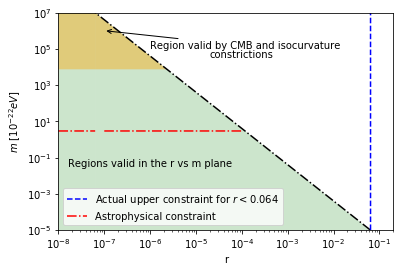
\includegraphics[width=8cm]{SFDMconstraints.png}
\caption{Isocurvature constraints for the SFDM candidate.}\label{constraintsSFDM}
\end{figure}\\

\textit{Massive complex SFDM model.-} A massive complex scalar field is described by the potential
\begin{equation}
V(|\psi|^2)= m^2|\psi|^2
\end{equation}
As we have shown in appendix [B] when we consider a complex scalar field its dynamics is modified only by the centrifugal term (see eq. \eqref{KGe3}). However as it was demostrated in \textcolor{red}{[referencias]} such term does not affect the dynamics of the field at cosmological levels, obtaining then that a complex scalar field and a real scalar field have the same cosmological history in the Universe. In this way if we consider that our complex SFDM fulfilled slow-roll conditions during inflation its constrictions for isocurvature perturbations must be the same than in the real field analogue. \\

\textit{Self-interacting SFDM scenario with a repulsive interaction.-} When the massive SFDM scenario is compared with observations there are several discrepancies about the constrictions for the mass of the model. For example when this model is tested at galactic levels by considering that its ground state of the self-gravitating BEC corresponds with the minimum DM halo, it is obtained a mass $m=2.92\times 10^{-22}eV$ for the SFDM model \cite{massconst1,SFphi42}; if in the other side the massive model is tested at cosmological levels considering big bang nucleosynthesis (BBN) constraints, it is obtained that $m>7.38\times 10^{-19}eV$ (see \cite{SFphi41,SFphi42}), which clearly is in disagreement with the constraints given by galactic scales. For this reason it is convenient to extend the model and introduce a self-interacting term that can help us to relax this discrepancies. For simplicity we continue considering that the SF does not interact with the inflaton in such case the total potential of the system can be given by
\begin{equation}
V(\phi,|\psi|^2)=V(\phi)+m^2|\psi|^2+\frac{1}{2}\lambda|\psi|^4
\end{equation}
As we have shown in appendix [B] we have 2 different scenarios in this model: a weak interacting and a strong interacting scenario. In the weak interacting model our SFDM behaves effectively as a massive field without auto-interaction, in such case the constrictions obtained by the massive field applies to this scenario. In the other side when the auto-interacting term is big enough we obtain that in the cosmological history of the scalar field we will have a new period where the SFDM behaves as a radiation-like fluid. In this way the constrictions that we have done before will not apply to this model anymore.

Before to start to study the strong scenario notice that we can give general constrictions for the auto-interacting term in terms of the ones that we have made until now. As we can see in appendix [B] we have the weakly self-interacting regime when $m^2\gg \lambda|\psi_i|^2/2$. In fact, thanks to the decreasing behavior of bout scenarios we can consider that this regime is fulfilled always that $m^2\geq \lambda|\psi_i|^2/2$ or equivalently when $\lambda\leq 2m^2/|\psi_i|^2$. If we consider that the SFDM oscillations start at the same moment that the only massive case (which is not really true but we can consider it as a good approximation), using eq. \eqref{phi_im2} we observe that this constriction can be given only in terms of the mass $m$ of the SF as
\begin{equation}
\left(\frac{\lambda}{10^{-96}}\right)\leq 1.2\left(\frac{m}{10^{-22}eV}\right)^{5/2}
\end{equation}
We plot in figure \ref{weekregime} the weak limit obtained by our approximation. However this limit overestimate the value of $\lambda$ since when in the above expression we have an equality the field is not behaved as a dust-like field at all, this behavior is obtained when the $\lambda$ term is completely negligible.
\begin{figure}
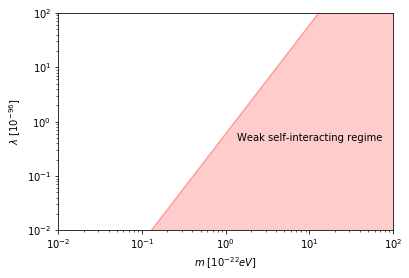
\includegraphics[width=8cm]{weakregime.png}
\caption{Weakly self-interacting regime}
\label{weekregime}
\end{figure} 

In the strong self-interacting regime the SFDM follows an attractor solution \eqref{atractor} during inflation (see appendix [B]) 
\begin{equation}\label{atractor0}
\eta_{att} =\left(2\lambda\int_{\phi}^{\phi_0}V^{-1}_{,\phi}d\phi\right)^{-1/2}
\end{equation}
Then the value that the homogeneous field can obtain after inflation depends on if $\eta_{att}<\sqrt{2}m/\sqrt{\lambda}\equiv \eta_t$ or not, where $\eta\equiv |\psi|$. When $\eta_{att}<\eta_t$ the field follows the attractor solution until $\eta\simeq \eta_t$. Then the scalar field is frozen at that value and starts to oscillate as a massive field when $m\sim H$. 

Notice that we can do two kind of constrictions of our free parameters. First, from equation \eqref{initial_c} and taking $|\psi_i|=\eta_t$ we have
\begin{equation}
r<1.2\times 10^{-4}\left[\frac{\left(\frac{m}{10^{-22}eV}\right)^2}{\frac{\lambda}{10^{-96}}}\right]
\end{equation}
While in the other side given the fact that when the SFDM starts its oscillations it behaves as a massive field, the constrictions obtained in the non-interacting field must be fulfilled as well. Matching $\eta_t$ with \eqref{phi_im2} and considering the constriction given in primordial tensor perturbations by eq. \eqref{constm} we obtain
\begin{equation}
\left(\frac{\lambda}{10^{-96}}\right)\leq 1.2\left(\frac{2\times 10^{-4}}{r}\right)^5
\end{equation}
In figure \ref{constraintsSFDMl} we have plotted the above condition that is valid in the weak interacting regime.

\begin{figure}[h]
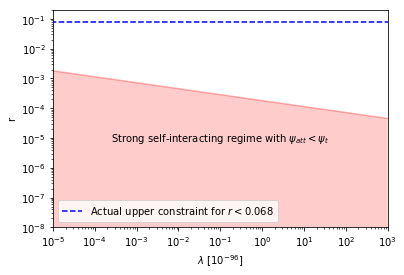
\includegraphics[width=8cm]{lambdavsr.png}
\caption{Isocurvature constraints for the weakly self-interacting term.}\label{constraintsSFDMl}
\end{figure} 

Additionally we can do more constraints for the inflationary potential in this scenario. Notice that it is fulfilled always that
\begin{equation}
\left(\int^{\phi_0}_\phi V_{,\phi}^{-1}d\phi\right)^{-1/2}<2m
\end{equation}
We can see that it is very difficult to obtain this relation for an ultra-light SFDM candidate. For example, if we consider a chaotic-like inflationary potential, $V(\phi)=\frac{1}{2}M_{inf}^2\phi^2$, the above conditions implies that
\begin{equation}\label{chaoticweek}
\left(\log\frac{\phi_0}{\phi}\right)^{-1/2}<2\frac{m}{M_{inf}}
\end{equation}
However, in a chaotic-like inflationary potential the mass $M_{inf}$ of the inflaton allowed that best matches the observations\footnote{This chaotic-like inflationary potential is ruled-out now for observations, however we use it as an example in order to obtain general constraints for our models.} is of order $M_{inf}\sim 10^{12} GeV$ \cite{Liddle}. If now we consider an ultra-light SFDM candidate with a mass $m\sim 10^{-22}eV$, the above conditions implies that the logarithmic part of the expression should be lower that $\sim 10^{-43}$. The inflationary behavior for a chaotic-like inflaton ends when $\phi_{end}\simeq 2M_{pl}$ \cite{curvatonatractor,Liddle}. In the other side as it is explained in \cite{curvatonatractor}, the initial condition of the inflaton can no be arbitrarily large since the stochastic behavior is significant for $\dot\phi H^{-1}<H/2\pi$. If it is considered that the Universe starts when the inflaton escapes from the stochastic behavior we have that the initial condition for the inflaton should be
\begin{equation}\label{phi_0}
\phi_0\sim 10^5\times M_{pl}\left(\frac{10^{13}GeV}{M_{inf}}\right)^{1/2}
\end{equation}
where we can easily see that the condition given in \eqref{chaoticweek} can not be fulfilled.

When $\eta_{att}>\eta_t$ we have that the field follows the attractor solution during all the period of inflation. In this way the initial condition that the SFDM obtains is given by \eqref{atractor2}
\begin{equation}\label{atractor3}
\eta_{att}^i = \left(2\lambda\int_{\phi_{end}}^{\phi_0}V^{-1}_{,\phi}d\phi\right)^{-1/2}
\end{equation}
Then the SFDM remains frozen at value $\eta_{att}^i$ until $M\sim H$ and then it start to oscillate with a quartic potential. In this scenario the SF density behaves as $\rho_{SFDM}\propto |\psi|^4$ in such case we can write $P_{SFDM}=4\delta\psi/\psi_i$. In this way the primordial isocurvature perturbations for a strong-interacting SFDM is given by
\begin{equation}
P_{SFDM}(k)=\left|\frac{2H_*}{\pi\psi_i}\right|^2
\end{equation}
In appendix [B] we show how the initial condition can be related with the value of the field that we see now. Using eqs. \eqref{inilamb2} and \eqref{phi_im2}, using $g_{*osc}=3.36$ and $g_{s*osc}=3.91$  and considering the appropiate constrictions equivalent that the ones obtained in \eqref{initial_c} we obtain
\begin{equation}\label{constr4}
r<\frac{1.172\times 10^{-4}}{7^{1/3}f^2(\sigma)}\left[\frac{2\left(\frac{m}{10^{-22}eV}\right)^{3/2}}{\left(\frac{\lambda}{10^{-96}}\right)}\right]^{1/2}
\end{equation}
We show in figure \ref{constraintsSFDMls} constraints obtained for the strong scenario in terms of tensor-to-scalar ratio. We plotted contours of the value of the right side on the above equation. Notice that the gray region in the figure corresponds with values larger that $0.1$ which are the currently upper limit for r. This implies that such region is already allowed by the model. It is necessary to mention that there are some region of parameters where the strong and the weakly scenarios are overlapped in our approximations. This is because the different simplifications that we had consider for our analysis. However this descriptions can give us general considerations for our SFDM models. For example, as we can see in the figure as long as the mass parameter $m$ of the SF decreases, the possible values of the auto-interacting parameter is less restrictive. In the other side, we can see that if we fix a mass $m$, it is possible to avoid isocurvature perturbations by increasing the value of the auto-interacting term until a lower value. For example, lets suppose that we are interested in a model with a mass $m\sim 10^{-21} eV$ in the strong regime. Let us assume as well that future experiments on gravitational waves measure $r\sim 0.05,0.01,0.001$. In this way we can see from figure \ref{constraintsSFDMls} that such observation should implies that $\lambda>10^{-94},10^{-95},10^{-97}$, where the last constriction is obtained by the lower value for $\lambda$ in the strong scenario.   
\begin{figure}
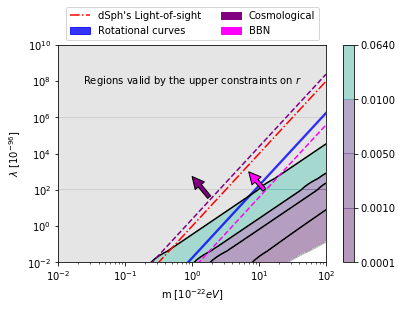
\includegraphics[width=8cm]{stronglamb.png}
\caption{Isocurvature constraints for the strong auto-interacting scenario.}\label{constraintsSFDMls}
\end{figure} 

Remark: This scenario is of special interest given that the attractor solution justify the initial conditions for the SFDM model and because it is natural to avoid isocurvature perturbations when the autointeracting term of the SF is big enough. 

Similar than in the above description we can do general constraints for the inflationary potential that should generate inflation on this kind of scenarios. First we can see that it must happen that
\begin{equation}
\left(\int^{\phi_0}_\phi V_{,\phi}^{-1}d\phi\right)^{-1/2}>2m
\end{equation}
which is very easy to fulfilled as we saw in the chaotic-like example. This relation can be translated into constrictions in the tensor-to-scalar ratio as
\begin{equation}
r<\frac{0.6\times 10^{40}}{\left(\frac{\lambda}{10^{-96}}\right)}\left(\frac{1}{\int_{\phi_{end}}^{\phi_0}V_{,\phi}^{-1}d\phi}\right)
\end{equation}
that can also be easily fulfilled always that the auto-interacting term and the integral are not extremely big; for example in the chaotic-like scenario by using \eqref{chaoticweek} and \eqref{phi_0}
%\begin{equation}
%\left(\int^{\phi_0}_\phi V_{,\phi}^{-1}d\phi\right)^{-1/2}\simeq (0.7403)\times 10^{21}
%\end{equation}
and taking $M_{inf}\simeq 10^{-6}M_{pl} $, we can obtain the constriction
\begin{equation}
\left(\frac{\lambda}{10^{-96}}\right)<\frac{0.3288\times 10^{84}}{r}
\end{equation}

If now we compare \eqref{atractor2} and \eqref{inilamb2} we have
\begin{equation}\label{inilamb3}
\left(\int_{\phi_{end}}^{\phi_0}V^{-1}_{,\phi}d\phi\right)^{-1}=\frac{6}{7^{1/3}f^2(\sigma)}\left(2m^2\lambda|\psi_t|^2\right)^{1/2}
\end{equation}
This relation can be interpreted as follows: consider that we are interested in an auto-interacting SFDM candidate that coexist with the inflaton. Suppose we have several measurements that constraints the mass parameter $m$ of the model as well as the auto-interacting one. In this way we can see that such constraints can be translated into constraints to the inflationary potential that causes inflation.  

It is also necessary to be careful that the SFDM does not come to dominate the inflationary period.  This is guarantee by demanding that
\begin{equation}
\lambda < \frac{H_*^2 M_p^2}{|\psi_i|^4}
\end{equation}
Or in terms of \eqref{atractor0}
\begin{equation}
\lambda>\left(4H_*^2M_{pl}^2\left(\int_{phi_{end}}^{\phi_0}V_{,\phi}^{-1}d\phi\right)^2\right)^{-1}
\end{equation}
Considering again the chaotic-like example and using $H_*= 10^{14} GeV$, we obain the constriction
\begin{equation}\label{lowerlambda}
\lambda > 5.777\times 10^{-19}
\end{equation}p=1,2,3,4,5,6

\textit{Different constraints for the self-interacting SFDM model}

This auto-interacting model can be tested at galactical levels by considering that its ground state corresponds with the minimum galaxy halo (Fornax) \cite{SFphi42}. With such observations we can constraint the ratio $\lambda/m^2$. If additionally we use constraints obtained by the Bullet Cluster \cite{bullet} it is possible to set the free parameters of the model. In \cite{SFphi42} it was obtained that for a strong self-interacting SFDM model we have
\begin{equation}
m= 1.10\times10^{-3}eV, \ \ \ \ \lambda = 2.46\times 10^{-17}
\end{equation}
while for a week self-interacting model we obtain
\begin{equation}
m= 2.92\times 10^{-22}eV
\end{equation}
This results corresponds with lower and upper bounds of the mass of the SFDM. In this way the mass of the SFDM should be in the range $2.92\times 10^{-22}\leq m\leq 1.10\times 10^{-3}eV$.

In the other side when the model is tested at cosmological levels using the CMB and the abundances of ight elements produced by the BBN it is obtained the values \cite{SFphi41,SFphi42}
\begin{equation}\label{masslamb}
m=3\times 10^{-21}eV, \ \ \ \ \ \lambda = 1.69\times 10^{-87}
\end{equation}
Notice that this last expressions are in agreement with the ones given by galactic constrictions.

If we consider \eqref{masslamb} as the most acceptable values for the mass of the SFDM and its auto-interacting term we can easily see from figure \ref{weekregime} that we should be in the strong regime. Then in this scenario the constrictions given in Eq. \eqref{constr4} (or equivalentily in figure \ref{constraintsSFDMls}) should apply. We observe in figure \ref{constraintsSFDMls} that the parameters obtained by BBN are easily acepted by the model due to the fact that those parameters are in the region that are already completely allowed by the constraints in the measurement on tensor-to-scalar ratio (grey region on the figure) which implies that the isocurvature perturbations are small enough that can avoid actual upper restrictions. In this way isocurvature perturbations does not represent any problem for the autointeracting model that matches with cosmological and galactical constrictions.

In the other side we can see that this parameters does not matches with lower constraints obtained in \eqref{lowerlambda}. This not represent a problem for auto-interacting SFDM models since that restriction was obtained for a chaotic-like inflationary potential and, as we already know, that inflationary model is ruled-out by the actual constraints given by Planck.

\subsection{Comments on Curvaton scenarios}

In the curvaton scenario it is assumed that during inflation there was an extra scalar field that coexist with the inflaton and its classical dynamics was negligible (its energy density was sub-dominant during inflation). Then, similar to the SFDM scenario, this SF obtained quantum fluctuations. If the curvaton field is long lived (at least its life must be longer than the inflaton one) it starts to oscillate when the Hubble scale $H$ approaches the curvaton mass shortly before or after the inflaton decays to radiation. During its oscillation phase, this curvaton field starts to behave as dust and then its energy density decreases slower than the ones associated with the inflaton (see appendix [C] for a review of the model). If the curvaton decays to radiation when its quantum fluctuations dominates over the inflaton ones, we can obtain a scenario where curvaton quantum fluctuations can dominate the early Universe and give place to be the totality of the initial adiabatic perturbations. In the formalism showed in \ref{Generalities} and as it is explained in \cite{twofields}, such scenario is obtained when $T_{RS}>>1$ or equivalently when we consider in our analysis $\sin\Delta = 0$, in such case we obtain that the tensor-to-scalar ratio in the pure curvaton scenario is $r=0$. 

There are also generation of isocurvature fluctuations on this scenario given by equation \eqref{PsAs}. Such fluctuations can be generated always that the DM or baryons were generated before the decay of the curvaton or for the decay products of the curvaton \cite{curvaton9,curvaton10,curvaton11}. To be preciss depending on how various particle numbers were generated they will inherit the curvaton, the inflaton or the total curvature fluctuations. For example, following \cite{curvaton12,curvaton13,curvaton14}, if the bariones or DM where created before the curvaton decays then they inherit inflaton's fluctuations, $P_R^\psi$. If they where generated by curvaton decays, they inherit the curvaton's fluctuations, $P_R^\sigma$. If they where generated before the curvaton decays they inherit the total curvature perturbation $P_R$. If they where generated after curvaton decays, isocurvature perturbations are not produced. There are other possibilities where one of the components where generated after curvaton decays and the other by, in such case every fluid inherit a different curvature perturbation, or the possibilty that compensated isocurvature perturbations \cite{curvaton14} were generated by all the processes mentioned before. Depending on the momment when baryons and DM where generated we will have several scenarios that can fulfilled actual constraints or not (see table I of reference \cite{curvaton14}). In this section and in order to simplify our analysis, we consider that we are already in a scenario where isocurvature perturbations satisfies observations. Additionally we consider that the total inflationary potential can be written as $V(\psi,\sigma)=V(\psi)+V(\sigma)$ wich implies that the fields are not correlated and then correlated fluctuations \eqref{PrCrs} are not generated. 

In the last few years researchers have started to study curvaton models but considering that the curvaton field does not constribute for the totality of the primordial adiabatic perturbations, instead, it contributes to a fraction of them, while the remaining one is produced by the inflaton \cite{curvaton4,curvaton5,curvaton6,curvaton7,curvaton8} (or for a more resent study see \cite{curvaton3}). This scenario is the so-called \textit{mixed inflationary model}. Notice that such scenario is obtained if $0<\cos\Delta <1$. It is also usual to redefine a new parameter in this model $\hat R= [\cot^2\Delta]_{k_0}$ which can be related with the curvaton-to-inflaton density fraction of primordial curvature perturbations. Then, the primordial curvature perturbations can be written from \eqref{PrAs} as
\begin{equation}\label{PCr}
\mathcal{P}_R(k)=A_r\left(\left(\frac{k}{k_{0}}\right)^{n_s^\phi-1}+\hat R\left(\frac{k}{k_{0}}\right)^{n_s^\sigma-1}\right)
\end{equation}
where $n_s^\phi-1 = -6\epsilon_\phi+2\eta_{\phi\phi}$ and $n_s^\sigma-1 = -2\epsilon_\sigma+2\eta_{\sigma\sigma}$.
The total spectral index ($n_s-1=d\ln P_R/d\ln k$) is given then by
\begin{equation}
n_s-1=\frac{n_s^\phi+\hat R n_s^\sigma}{1+\hat R}-1
\end{equation}
From \eqref{Tensortoscalar} the tensor-to-scalar ratio in this model is given by
\begin{equation}\label{tensortoscalar}
r=\frac{16\epsilon_\phi}{1+\hat R}
\end{equation}		
We can notice then that depending on the value of $\hat R$ we can obtain different values for the inflationary observables. When $\hat R=0$ we obtain the inflation scenario, whereas if $\hat R\gg 1$ we obtain the pure curvaton scenario.  

The possible values that $\hat R$ can obtains depend on the particular model of inflation, the value that the curvaton had during inflation and its evolution history (see appendix [C] and equation \eqref{R_r}). In particular it depends linearly on $\epsilon_\psi$, which implies that the larger $\epsilon_\psi$ is, the larger the curvaton contribution. For example, for large field inflationary models the curvaton can contribute more to the primordial curvature perturbations, while for small field models, the curvaton contributes less. This result is very convenint because large-field models usually predict large tensor-to-scalar ratio observations, while last observations allow small $r$ \eqref{Tensortoscalar}. In this way we notice that the addition of a new free parameter can help to relax different inflationary models.  

In \cite{curvaton15} it was studied chaotic-like inflationary models with an extra light scalar field. In such study it was obtained that one of the most preferable scenarios is a quartic-like inflationary potential with our extra scalar spectator. However it is necessary to notice that such scenario is favorable only when the mass of the curvaton can be negligible compared with the Hubble parameter. For the main porpoise of this article we can consider that example and observe how the inflationary parameters are predicted by the model. In fact when we consider the chaotic potential $V(\phi)=(1/2)\lambda_p\phi^p$ for the inflaton and the  potential $V(\sigma)= (1/2)M^2\sigma^2$ for the curvaton, the spectral index $n_s$ is rewritten as
\begin{equation}
\label{nsexplicit}
n_s-1\approx -\frac{1}{1+\hat R}\frac{2(2+p)}{4N+p}+\frac{\hat R}{1+\hat R}\left[-\frac{2p}{4N+p}+\frac{2M^2}{3H_*^2}\right]
\end{equation}
where  $N$ is the number of e-folds produced before our scales left the horizon and it is usually used $N=50\sim 60$. In the above equation we have used the Friedman equation in the slow-roll approximation for the term containing $M$. If we use \eqref{tensortoscalar} into \eqref{nsexplicit} we have 
\begin{equation}
n_s-1=-\frac{(2+p)}{8p}r+\left[1-\frac{(4N+p)}{16p}r\right]\left[\frac{2}{3}\frac{M^2}{H^2}-\frac{2p}{4N+p}\right]
\end{equation}
where we have obtained a relation between the spectral index and the tensor-to-scalar ratio which are well constrain by the data. Notice that in the limit when the curvaton dominates completely the adiabatic perturbations ($r\simeq 0$) and considering the mass of the curvaton negligible compared with the Hubble parameter (i.e. $M<<H$) we obtain that $n_s-1\simeq p/(120+p/2)$ and then the observational constrains for the spectral index \eqref{n_R } means that the inflaton field must be close to be a quartic potential, $p=4$. Such result can be observed in figure \ref{nvsr}, where we have plotted the above equation neglecting $M/H$ and letting $R$ to vary using as our only constriction for it the actual upper constraint on $r$. In such figure we can observe an upper an lower value for $n_s$ in terms of $r$ which is obtained when we consider $N=60-50$ e-folds at the moment when our scales left the horizon. In the other side we could consider the next level of complication allowing $M/H$ to vary using as our constriction that $M/H<1$ (in order to obtain quantum fluctuations for the curvaton during inflation), considering that the curvaton never dominates during the inflationary era, which is guarantied when
\begin{equation}\label{MoverH}
\frac{M^2}{H^2_*}<\frac{M_{pl}^2}{\sigma_i^2}
\end{equation} 
and that its oscillations starts after inflaton oscillations, which implies
\begin{equation}\label{M2curv}
M^2\lesssim p(p-1)\lambda_p \psi_{end}^{p-2}
\end{equation}
where $\psi_{end}$ is the value of $\psi$ at the end of inflation. We can see from \eqref{R_r} that $(M_{pl}^2/\sigma_i^2)\sim R/\epsilon r_{dec}^2$. In a typical scenario $r_{dec}^2\ll 1$, while $\epsilon\ll 1$ by slow-roll construction. Then, if we allow $\hat R$ to be big enough (we are not in the just inflationary scenario) expression \eqref{MoverH} is fulfilled trivially when we demmand $M/H<1$. Inflaton oscilations starts inmediatelly after inflations ends, then we can consider that $0<M^2/H^2<1$. In figures \ref{curv50} and \ref{curv60} we have plotted contour regions for $r$ in the plane $n_s vs M^2/H^2$ in the range $10^{-5}<M^2/H_*^2<0.5$, for $N=50,60$ and for $p=1,2,3,4,5,6$. As we can see when only $r$ and $n_s$ are consider it looks that quartic and cubic potentials can fit well observations. For the typical quadratic and the linear potentials we can see that we can obtain parameters that are inside actual bonds on the parameters but only by obtaining relatively large $r$. For the last two potentials it is also possible to obtain the observations required but only when $M/H$ is not so small and for a very little region of parameters.   
\begin{figure}
\centering
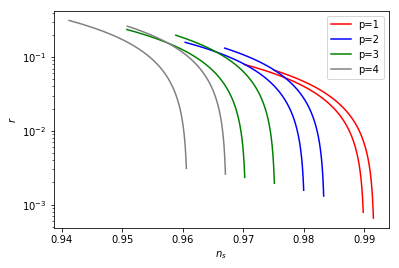
\includegraphics[width=0.4\textwidth]{nvsr}
\caption{Possible values in the n vs r plane when we allow $R$ to vary. The values that can be produced by the models are the ones between the two limits plotted in the figure.\textcolor{red}{(Tratar de pintar las regiones entre las l\'ineas y poner los datos de Planck para que se vea mejor.)}}
\label{nvsr}
\end{figure}
% * <epadilla@fis.cinvestav.mx> 2018-04-29T03:33:02.572Z:
%
% ^.
\begin{figure}[h!]
\raggedright
\begin{subfigure}[b]{0.6\textwidth}
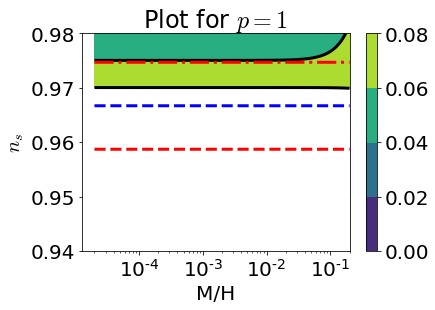
\includegraphics[width=0.3\textwidth]{p150.png}
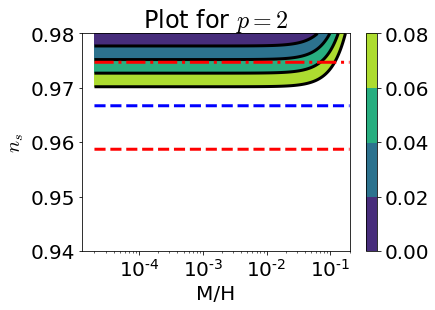
\includegraphics[width=0.3\textwidth]{p250.png}\\
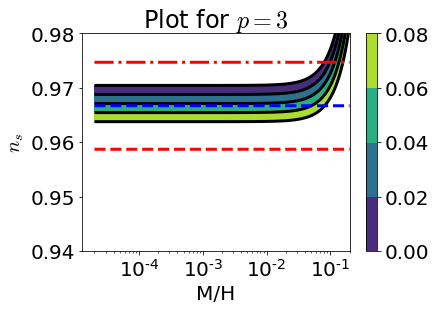
\includegraphics[width=0.3\textwidth]{p350.png}
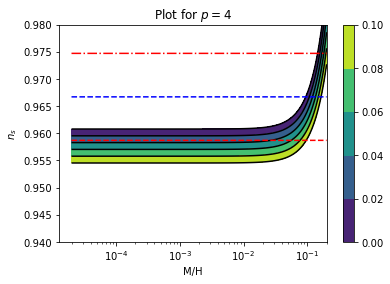
\includegraphics[width=0.3\textwidth]{p450.png}\\
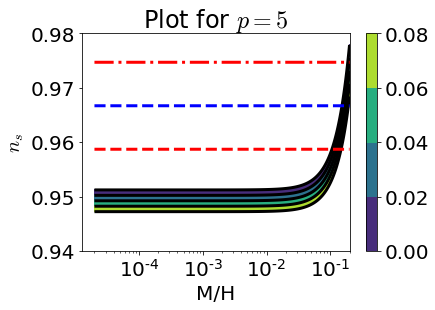
\includegraphics[width=0.3\textwidth]{p550.png}
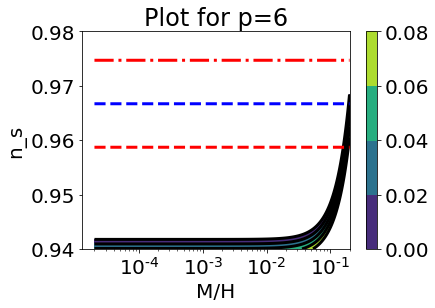
\includegraphics[width=0.3\textwidth]{p650.png}
\label{curv50}
\end{subfigure}
\caption{Inflationary constraints in the $M/H$ vs $n_s$ plane for $N=50$ e-folds. We plotted contour regions for $0<r<0.1$.}
\begin{subfigure}[b]{0.6\textwidth}
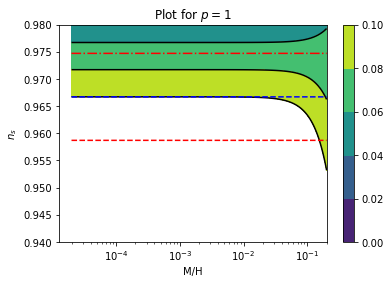
\includegraphics[width=0.3\textwidth]{p160.png}
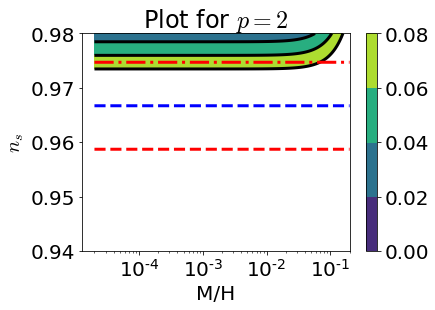
\includegraphics[width=0.3\textwidth]{p260.png}\\ 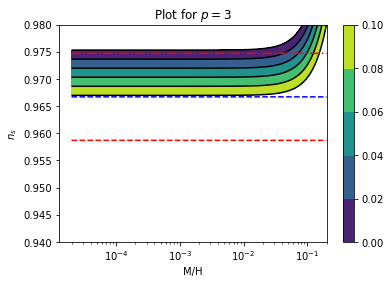
\includegraphics[width=0.3\textwidth]{p360.png}
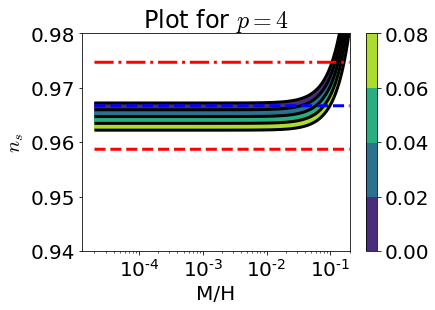
\includegraphics[width=0.3\textwidth]{p460.png}\\
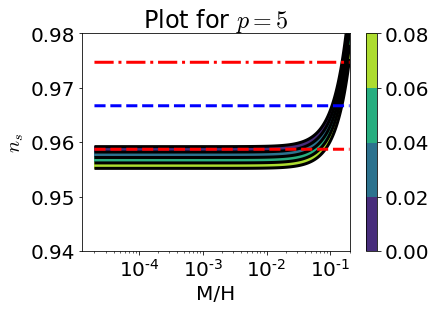
\includegraphics[width=0.3\textwidth]{p560.png}
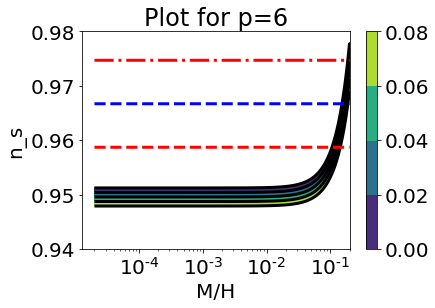
\includegraphics[width=0.3\textwidth]{p660.png}
%\captionof{figure}
%{\footnotesize{A }}
\label{curv60}
\end{subfigure}
\caption{Inflationary constraints in the $M/H$ vs $n_s$ plane for $N=60$ e-folds. We plotted contour regions for $0<r<0.1$.}
\end{figure}
\section{Constraining curvaton models with last data}
\textcolor{red}{(Esta ser\'ia tu parte, Beto)}
\section{Conclusions}
\appendix
\section{Slow-Roll index}

In this appendix we define the slow roll indexes used in our calculation. We have:
\begin{subequations}
\begin{equation}
\epsilon_i = \frac{1}{16 \pi G}\left(\frac{V_i}{V}\right)^2, \ \ \ \ \ \text{where $i=\phi,\psi$}
\end{equation}
\begin{equation}
\eta_{ij}=\frac{1}{8\pi G}\left(\frac{V_{ij}}{V}\right)
\end{equation}
\end{subequations}
where $V_i = \partial V/\partial \phi_i$. In the other side we have
\begin{equation}
\epsilon \equiv \frac{1}{16\pi G}\left(\frac{V_\sigma}{V}\right)^2\simeq \epsilon_\phi+\epsilon_\psi
\end{equation}
and
\begin{eqnarray}
\eta_{\sigma\sigma}&=&\eta_{\phi\phi}\cos^2\theta + 2\eta_{\phi\psi}\cos\theta\sin\theta+\eta_{\psi\psi}\sin^2\theta\nonumber \\
\eta_{\sigma s}&=&(\eta_{\psi\psi}-\eta_{\phi\phi})\sin\theta\cos\theta + \eta_{\phi\psi}(\cos^2\theta-\sin^2\theta)\\
\eta_{ss}&=&\eta_{\phi\phi}\sin^2\theta - 2\eta_{\phi\psi}\cos\theta\sin\theta+\eta_{\psi\psi}\cos^2\theta\nonumber 
\end{eqnarray}
\section{Generalities for SFDM models}

In order to constraint our SFDM model using our isocurvature constrictions it is necessary to relate the value of the field now with the value that it has during inflation. This constrictions depend on the SFDM model that we consider. In this appendix we analyze the evolution of different models for SFDM and then in [section], with the help of isocurvature constrictions, try to constraint the free parameters of our models. 

In this scenario our scalar field can be coupled or not with the inflaton, then we consider the general potential of the form $V(\phi,|\psi|^2)$, where in such case it is convenient to work using a Madelung transformation \eqref{madelung}
\begin{equation}
\psi = \eta \exp[i\theta]
\end{equation}
where $\eta\equiv |\psi|$ is the magnitude of field $\psi$ and $\theta$ its phase. Notice that in order to obtain a slow-roll approximation it is neccesary that $|\theta|<<1$ and $\eta$ fulfill the slow-roll condition during inflation. Since we are interested in the complete history of the SFDM in the Universe let us rewrite and separate the KG equation in its real and imaginary components as
\begin{subequations}\label{KESFDM}
\begin{equation}\label{KGe1}
\ddot\eta+3H\dot\eta+\frac{dV}{d|\psi|^2}\eta-\omega^2\eta= 0,
\end{equation}
\begin{equation}\label{KGe2}
\dot\omega \eta + (2\dot\eta+3H\eta)\omega=0
\end{equation}
\end{subequations}
where $\omega = \dot \theta$, while the equation of the inflaton field continue being eq. \eqref{KGEq}. Equation \eqref{KGe2} can be exactly integrated as
\begin{equation}
\frac{d}{dt}\left(a^3\eta^2\omega\right)=0
\end{equation}
wich implies that 
\begin{equation}
a^3\eta^2\omega=Q
\end{equation}
where $Q$ is a charge of the SF related with the total number of particles \cite{SFphi42,charge1,charge2,charge3,charge4}. Using this last equation in \eqref{KGe1} we obtain finally
that the radial component of the scalar field fulfill
\begin{equation}\label{KGe3}
\ddot\eta+3H\dot\eta+M^2\eta-\frac{Q^2}{\eta^3}= 0,
\end{equation}
The term containing $Q$ is obtained by the complex nature of the SF [ref] an it can be interpreted as a "cenrifugal force" [ref]. In the other side $M\equiv dV/d|\psi|^2$ can be interpreted as an effective mass term of the scalar field. Notice here that if we consider $Q^2/\eta^3\ll 1$ and we suppose that the SFDM candidate fulfill the slow-roll condition during inflation, the field $\eta$ will remain frozen at value $\eta_i$ until $H\sim M$. Then, when $H\sim M$ it will start to evolve depending on the behavior of the effective mass term.
\begin{center}
\textit{A real massive SFDM candidate}
\end{center}

A massive real scalar field is described by the potential 
\begin{equation}
V = \frac{1}{2}m^2\psi^2
\end{equation}
Then we have that in equations \eqref{KESFDM} $\eta=\psi$ and $\theta=0$ which implies that $\omega=0$ and then $Q = 0$. We consider for simplicity that our SFDM candidate was not coupled with our inflaton field, in such case we can rewrite the total potential during inflation as

\begin{equation}
V(\phi,|\psi|^2)=V(\phi)+\frac{1}{2}m^2\psi^2
\end{equation}
In this way we can see that $M^2=m^2$. As we mentioned above when $H\gg m^2$ the therm that contains $m^2$ in equation \eqref{KGe1} can be neglected. Since we are considering that the field is slowly rolling during the inflationary era, we can neglect the second derivatives in \eqref{KGe1}\footnote{In fact the inflationary behavior is an attractor solution of the KG equation in the limit when $M^2<<H^2$ \cite{atractorinf1,atractorinf2}. The typical dynamics of a real SF in this limit is a stiff-like era followed by a inflationary-like era. In this article we consider that during the period of inflation that we are interested the SFDM candidate was in the inflationary-like era.}, then the field $\psi$ remains frozen at its initial value by Hubble dragging during the early universe \cite{curvatonatractor}. Then, when $m\sim H$ the SFDM starts to evolve and oscillate as a massive field. During its oscillation phase the dependence of $\psi$ respect to $a$ is $\psi\sim 1/a^{3/2}$, while its density behaves as $\rho_{\psi}\sim 1/a^3$  \cite{SFphi41,SFphi42}. In this way we can write the scalar density of our field as
\begin{equation}\label{rhosfdm}
\rho_\psi = \left\lbrace\begin{array}{ll}
\frac{1}{2}m^2\psi_i^2 & \text{when }H\gg m \\
\frac{1}{2}m^2\psi_i^2\left(\frac{a_{osc}}{a}\right)^3 & \text{when }H\ll m
\end{array}\right .
\end{equation}

The typical mass that it is considered for a SFDM candidate is around $10^{-22} eV$ which implies that the field should starts its oscilations during a radiation-dominated Universe. During this period the Hubble parameter evolves in terms of the scale factor as $H\propto a^{-2}$. We can solve the KG equation \eqref{KGe1} exactly during this period in terms of the scale factor obtaining
\begin{equation}
\psi = \psi_i\Gamma\left(\frac{5}{4}\right)\left(\frac{4H}{m}\right)^{1/4}J_{1/4}\left(\frac{m}{2H}\right)
\end{equation}
where $\psi_i$ is the scalar field value during inflation and it was imposed initial condition for $\psi$ in such a way that when $m/H\rightarrow 0$ we obtain $\psi\rightarrow\psi_i$. If now we consider that in the above expression we obtain the $H\ll m$ behavior of equation \eqref{rhosfdm} when $m/H\rightarrow \infty$ we obtain that
\begin{equation}\label{m_osc}
\frac{m^2}{H_{osc}^2}\simeq 2.68
\end{equation}
whit $H_{osc}$ the value of the Hubble parameter at the momment when the SFDM starts its oscilations.

Using the relation for a radiation-dominated Universe
\begin{equation}
\rho_r = 3M_p^2H^2=\frac{\pi^2}{30}g_*T^4
\end{equation}
where $M_p\equiv (8\pi G)^{-1/2}$ is the Planck mass and $g_*$ the effective degrees of freedom, and \eqref{m_osc} we can obtain the temperature when our SFDM particle starts its oscilations
\begin{equation}
T_{osc}\simeq 0.5 keV\left(\frac{g_{*osc}}{3.36}\right)^{-1/4}\left(\frac{m}{10^{-22}eV}\right)^{1/2}
\end{equation}
where we have left the values inside the parentesis for $g_{*osc}$ and $m$ by convenience since our ultra-light particle starts its oscilations during a radiation-dominated era. 

Finally, using that the entropy of the Universe is conserved we can express the actual density of SFDM particles as
\begin{equation}
\rho_{DFDM}=\frac{1}{2}m^2\psi_i^2\frac{s_0}{s_{osc}}
\end{equation}
where the subscript ``$0$" indicates quantites at present. Using the relation that $s=\frac{2\pi}{45}g_{*}T^3$ and the constraints given by Planck \cite{Planckcolaboration} for the actual amount of Dark Matter content $\Omega_{DM}h^2=0.1186\pm 0.0020$ $68\% CL$, we finally obtain 
\begin{equation}\label{phi_im2}
|\psi_i|^2\simeq\frac{10^{34}GeV^2}{0.6}\left(\frac{g_{*osc}}{3.36}\right)^{-3/4}\left(\frac{g_{s*osc}}{3.91}\right)\left(\frac{m}{10^{-22}eV}\right)^{-1/2}
\end{equation}
The above expression coincide with the one obtained in \cite{SFrev2} where constraints for isocurvature perturbations and Lyman-$\alpha$ for a real massive SF was studied.
\begin{center}
\textit{A complex massive SFDM candidate}
\end{center}

Let us consider now a complex scalar field which is not coupled with the inflaton. This scenario is obtained by considering a complete potential of the form
\begin{equation}
V(\phi,|\psi|^2)=V(\phi)+m^2|\psi|^2
\end{equation}
We demand slow-roll for our complex scalar field which implies that the charge $Q$ of the scalar field must be small enough. Additionally, as we saw in the real case in order to avoid isocurvature perturbations it is neccesary that the scalar field starts from a high value of $\eta_i$ in such case we can ignore the last term in eq. \eqref{KGe3}. In the other side considering the same argument than in the real case we can see that the SF value remains frozen until $m\sim H$ and then it starts to oscilate. It is easy to see that given the above arguments a massive complex scalar field behaves equivalent to the real case at cosmological levels, being the $Q $ term important only at galactic levels \textcolor{red}{[ref]}. Taking this in mind we can consider that all what we did in the real case applies to this case and then a complex scalar field has the same constrictions than the real one. 
\begin{center}
\textit{Self-interacting Scalar Field with a positive interaction}
\end{center}

We consider in this section a self-interacting scalar field with a positive interaction. This scenario is described by the potential associated with the SFDM
\begin{equation}
V = m^2|\psi|^2+\frac{1}{2}\lambda |\psi|^4
\end{equation}
Again we consider that the charge $Q$ associated to the SFDM candidate is small enough in order to obtain the slow-roll era. If we consider that our SF was not coupled with the inflaton we will have that the complete dynamics of the system is obtained with the full potential 
\begin{equation}
V(\phi,|\psi|^2)=V(\phi)+m^2|\psi|^2+\frac{1}{2}\lambda|\psi|^4
\end{equation}
Notice that the effective mass of the field is $M^2=m^2+\lambda|\psi|^2$. Thanks to the slow-roll condition imposed during inflation the effective mass of the field after inflation remains constant at $M^2=m^2+\lambda|\psi_i|^2$ until $M\sim H$, then, depending on what term dominates in $M^2$ we can have two different kind of dynamics. 
\\

\textit{Weakly self-interacting regime.-} This limit is obtained when the constant term in $M^2$ dominates, it is when
\begin{equation}\label{consw}
m^2\gg \frac{1}{2}\lambda|\psi_i|^2
\end{equation}
In this regime it is possible to ignore the autointeracting term in equation \eqref{KGe3} when oscilations of the scalar field begins. However, because when we ignore such term the field behaves as a massive field and as we can see in \eqref{rhosfdm} the field value always decreases, the autointeracting term never dominates and then all the cosmological history of the SFDM candidate is the same than in the pure massive scenario. 
\\

\textit{Strong self-interacting regime.-} This scenario is obtained when 
\begin{equation}
m^2\ll \frac{1}{2}\lambda|\psi_i|^2
\end{equation}
In this scenario it happens that the SFDM follows an attractor solution during the inflationary era. In this way we will have two different scenarios depending the value of the attractor solution.
\\

\textit{Attractor behavior of the SF during inflation.-} In the strong self-interacting regime the SFDM follows the attractor solution \cite{curvatonatractor}
\begin{equation}\label{atractor}
\eta_{att} =\left(2\lambda\int_{\phi}^{\phi_0}V^{-1}_{,\phi}d\phi\right)^{-1/2}
\end{equation}
where $\phi_0$ is the value of the inflaton at the beggining of inflation. We can identify two possible scenarios in the above expression:
\begin{itemize}
\item $\eta_{att}<\sqrt{2}m/\sqrt{\lambda}$

In this scenario the SFDM follows the attractor solution until $\eta\simeq \sqrt{2}m/\sqrt{\lambda}$. Then the SF reaches $\eta_i=\sqrt{2}m/\sqrt{\lambda}$ for the rest of inflation. Notice that this value corresponds with the upper value that the weakly self-interacting regime allows. Then the field starts to evolve when $H\sim M\simeq m$ behaving as a massive SF. In this way, for this scenario, the constrictions given in the non-interacting case apply but where the initial condition are also fixed by $\eta_i$. Using both relations we can obtain the value that $\lambda$ should have, which is
\begin{equation}
\left(\frac{\lambda}{10^{-96}}\right)=1.2\left(\frac{g_{*osc}}{3.36}\right)^{3/4}\left(\frac{g_{s*osc}}{3.91}\right)^{-1}\left(\frac{m}{10^{-22}eV}\right)^{5/2}
\end{equation}\\

\item $\eta_{att}>\sqrt{2}m/\sqrt{\lambda}$

In this scenario the dynamics of the inflaton is given by \eqref{atractor} during inflation which implies that the initial condition of the field after inflation is given by
\begin{equation}\label{atractor2}
\eta_{att}^i = \left(2\lambda\int_{\phi_{end}}^{\phi_0}V^{-1}_{,\phi}d\phi\right)^{-1/2}
\end{equation}
where $\phi_{end}$ is the value of the inflaton at the end of inflation. We need to specify that it is the value of the field in the early Universe until its oscilations starts (i.e. $M\sim H$).

In this scenario we can see that at the moment when the SFDM starts its oscillations its effetive mass is quadratic in the field. In that regime the scalar field evolves as $\psi\sim 1/a$ and its energy density as $\rho_{\psi}\sim 1/a^4$ behaving as radiation. Then, when $m^2 \sim \frac{1}{2}\lambda|\psi_t|^2$ we obtain that the effective scalar field mass is now constant, obtaining the dust-like behavior that we analyze before. In this way we can write the history of the scalar density of our field as
\begin{equation}\label{rhosfdmlam}
\rho_\psi = \left\lbrace\begin{array}{ll}
\frac{1}{2}\lambda^2|\psi_i|^4 & \text{where }H\gg \lambda|\psi_i|^4 \\
\frac{1}{2}\lambda|\psi_i|^4\left(\frac{a_{osc}}{a}\right)^4 & \text{where }H_t\leq \lambda|\psi_i|^4\leq H\\
m^2|\psi_t|^2\left(\frac{a_t}{a}\right)^3 & \text{where } m^2\leq H_t
\end{array}\right .
\end{equation}
Here sub-index $t$ means quantities measured at transition between radiation and dust behavior of the SFDM and
\begin{equation}\label{inilamb}
|\psi_i|^2=\left[\frac{2m^2}{\lambda}|\psi_t|^2\right]^{1/2}\left(\frac{a_t}{a_{osc}}\right)^2
\end{equation}
Notice that we have consider for simplicity a direct transition between radiation-like to dust-like behaviors. 

In order to continue it is necessary to specify the value of $a_t$ and $a_s$. Since the auto-interacting KG equation can not be solved exactly it is necessary to work with approximated solutions. In \cite{SFphi42} (see also \cite{SFphi41}) it was obtained using a pure approximated description of the system the relation (see its equation 80 and 86)
\begin{subequations}
\begin{equation}\label{atoveras}
\left(\frac{a_t}{a_{osc}}\right)^2=\frac{3}{7^{1/3}f^2(\frac{a_s}{r_S})}
\end{equation}
where 
\begin{equation}
f(\sigma)=\frac{1}{s^{1/3}(1+4s)^{1/6}}
\end{equation}
with
\begin{equation}
s=\frac{4\sigma-1+\sqrt{(4\sigma-1)^2+12\sigma}}{6}
\end{equation}
\end{subequations}
Additionally $r_S=2mG/c^2$ and $a_s=\hbar^2\lambda/4\pi m$ which implies that $a_s/r_s=\lambda M_p^2/m^2$. Rearranging it in a more convenient way we have
\begin{equation}
\sigma \simeq 5.93\times 10^{
2}\left(\frac{m}{10^{-22}eV}\right)^{-2}\left(\frac{\lambda}{10^{-96}}\right)
\end{equation}
Notice that when $a_t/a_{osc}\simeq 1$ i.e. when $3/(7^{1/3}f^2(\sigma))\sim 1$ there is not a radiation-like epoch. This scenario should match with the non-interacting scenario that we studied before.

Inserting equation \eqref{atoveras} into \eqref{inilamb} follows
\begin{equation}\label{inilamb2}
|\psi_i|^2=\frac{3}{7^{1/3}f^2(\sigma)}\left[\frac{2m^2}{\lambda}|\psi_t|^2\right]^{1/2}
\end{equation}
But the above relation means that it is enough to match the value of the field at $\psi_t$ with the value at present and then with the above relation we can obtain the value that the SF had during inflation. In the other side notice that at $a_t$ the scalar field starts to behave as dust with an effective mass $M^2=m^2+\lambda|\psi_t|^2$. This implies that dust-like oscillations of the SF start a little before than the non-interacting case. If we allow $m$ to be ultralight $(m\sim 10^{-22}eV)$ and thanks to the fact that $m^2$ is of the same order that $\lambda|\psi_t|^2$ we can see that such oscillation starts at the same epoch that the non-interacting case does. In fact we can see that because the decreasing behavior of the SF at that period ($\psi\sim 1/a^{3/2}$) the auto-interacting term left to be important quickly and then the dynamics of the field is quickly described only by the mass term $m$. We consider for simplicity that once the dust-like behavior starts, the dynamics is described similar to  the non-interacting case, in such case the condition \eqref{phi_im2} is fulfilled by our SF as well, but interchanging subindex $i$ with $t$\footnote{In fact this is a lower boundary for the strong auto-interacting case.}.
\end{itemize}
\section{A review on the physics on Curvaton models}

The curvaton $\sigma$\footnote{We use $\sigma$ since it is the most commun way that the curvaton field is represented in literature} is a real light scalar field during inflation which starts to oscilate when the Hubble parameter approaches to its mass $m_\sigma$ shortly before or after the inflaton $\phi$ decays into radiation. It was propossed in \cite{curvaton1} as an alternative mechanism for generating the primordial density perturbation on the Universe. In the typical scenario the curvaton is assumed to be quadratic on its potential which implies that when its oscilations starts it behaves as a pressureless fluid. During its oscilation phase and considering that the inflaton has already decay we have that bouth fluids evolves as $\rho_\sigma\sim a^{-3}$ (dust-like evolution) an $\rho_{rad}\sim a^{-4}$ (radiation-like evolution). In this way we can see that during this period the curvaton energy density decreases slower than the inflaton one and then its fraction contribution for the total energy of the Universe can be larger and larger and generate curvature fluctuations \cite{curvaton1}.

In this scenario, the curvature perturbation $R$ evolves until the curvaton decays. Then $R$ stops evolving and becomes constant at the super-horizon scale. In the general scenario both fluids can be responsabble for the generation of the primordial curvature fluctuation $R$. If we assume that $\phi$ and $\sigma$ are uncorrelated, the power spectrum of curvature perturbations $P_R$ is given by
\begin{subequations}
\begin{equation}
P_R(k)=P_R^{(\phi)}(k)+P_R^{(\sigma)}(k)=(1+\hat R)P_R^{(\phi)}
\end{equation}
where $P_R^{(\phi,\sigma)}$ are the power spectra for the curvature perturbation generated by the field $\phi,\ \sigma$ and we have defined the ratio $\hat R$ between bout spetra as
\begin{equation}
\hat R\equiv \frac{P_R^{(\sigma)}}{P_R^{(\phi)}}
\end{equation}
\end{subequations}
The fraction $\hat R$ can be also related with the ratio $r_{dec}$ of curvaton energy $\rho_\sigma$ to radiation energy $\rho_{rad}$  at the time of the curvaton decay as
\begin{equation}\label{R_r}
\hat R =\frac{8}{9}\epsilon \left(\frac{M_{pl}}{\sigma_i}\right)^2 r^2_{dec}
\end{equation}
where $\sigma_i$ is the value of the curvaton during inflation and
\begin{equation}
r_{dec} =\left.\frac{\rho_\sigma}{\rho_\sigma + 4\rho_{rad}/3}\right|_{dec}
\end{equation}
Notice that the pure curvaton senario is obtained when $ R\gg 1$ and then the primordial curvature perturbations are generated only by $\sigma$.

When the curvaton decays and considering that the Universe is domminated by a radion-dominated era, $r_{dec}$ can be approximated as \cite{curvaton2,curvaton3}
\begin{equation}
r_{dec}\sim \left(\frac{\sigma_*}{M_{pl}}\right)^2\sqrt{\frac{m_\sigma}{\Gamma_{\sigma}}}
\end{equation}
where $\Gamma_\sigma$ is the decay rate for the curvaton.
\section{Papers} 
Aqu\'i pondré de mientras los links de los papers que he revisado:

https://arxiv.org/pdf/1211.3535.pdf

https://arxiv.org/pdf/1712.05364.pdf

https://arxiv.org/pdf/1505.00639.pdf

https://arxiv.org/pdf/astro-ph/0306500.pdf

https://arxiv.org/pdf/1708.05681.pdf

https://arxiv.org/pdf/1211.3535.pdf

https://arxiv.org/pdf/1507.00119.pdf

https://arxiv.org/pdf/1801.07409.pdf

https://arxiv.org/pdf/1305.5338.pdf

\begin{thebibliography}{9}
\bibitem{twofields} Christian T. Byrnes, David Wands;  Phys.Rev. D74 (2006) 043529; DOI:  	10.1103/PhysRevD.74.043529;  arXiv:astro-ph/0605679v3
\bibitem{const1}  P. A. R. Ade
et al.
(Planck), Astron. Astrophys.
571
, A16 (2014), arXiv:1303.5076 [astro-
ph.CO]
\bibitem{const2} ]  P. A. R. Ade
et al.
(Planck), Astron. Astrophys.
571
, A22 (2014), arXiv:1303.5082 [astro-
ph.CO]
\bibitem{planck} P. A. R. Ade et al. (Planck); DOI: 	10.1051/0004-6361/201525898;  	arXiv:1502.02114 [astro-ph.CO]
\bibitem{const3}  D. Barkats
et al.
(BICEP1), Astrophys. J.
783
, 67 (2014), arXiv:1310.1422 [astro-ph.C
\bibitem{const4} P. A. R. Ade
et al.
(BICEP2, Planck), Phys. Rev. Lett.
114
, 101301 (2015), arXiv:1502.00612
[astro-ph.CO]
\bibitem{const5}  P.  A.  R.  Ade
et al.
(BICEP2,   Keck  Array),  Phys.  Rev.  Lett.
116
,  031302  (2016),
arXiv:1510.09217 [astro-ph.CO]
\bibitem{H1}  D. Lyth, Physics Letters B
147
, 403  (1984)
\bibitem{H2}  D. H. Lyth and E. D. Stewart, Physics Letters B
283
, 189  (1992).
\bibitem{SF1} Baldeschi M., Gelmini G., Ruffini R., 1983, Phys.Lett.B, 12
\bibitem{SF2} Matos T., Guzman F. S., 2000, Class. Quant. Grav., 
\bibitem{SF3} Hu W., Barkana R., Gruzinov A., 2000, Physical Review Letters, 85, 1158
\bibitem{SF4}Bray H., 2010
\bibitem{SF5}Schive H.-Y., Chiueh T., Broadhurst T., 2014a, Nature Phys., 10, 496
\bibitem{SF6}Böhmer C. G., Harko T., 2007, J. Cosmology Astropart. Phys., 6, 025
\bibitem{SF7}Marsh D. J. E., Ferreira P. G., 2010, Phys. Rev. D, 82, 103528
\bibitem{SF8} Membrado M., Pacheco A. F., Sañudo J., 1989, Phys.Rev.A, 39, 4207
\bibitem{curv1}K. Enqvist and M. S. Sloth, Nucl. Phys. B
626
(2002) 395 doi:10.1016/S0550-3213(02)00043-3
[hep-ph/0109214
\bibitem{curv2}D. H. Lyth and D. Wands, Phys. Lett. B
524
(2002) 5 doi:10.1016/S0370-2693(01)01366-1
[hep-ph/0110002
\bibitem{curv3} T. Moroi and T. Takahashi, Phys. Lett. B
522
(2001) 215 [hep-ph/0110096]
\bibitem{madelung}  E. Madelung, Zeit. F. Phys.
40
, 322 (1927)
\bibitem{atractorinf1}  V.A.  Belinsky,  L.P.  Grishchuk,  I.M.  Khalatnikov,  and
Ya.B. Zeldovich, Phys. Lett. B
155
, 232 (1985)
\bibitem{atractorinf2}  T.  Piran  and  R.M.  Williams,  Phys.  Lett.  B
163
,  331
(1985)
\bibitem{SFphi41}  B. Li, T. Rindler-Daller, and P.R. Shapiro, Phys. Rev.
D
89
, 083536 (2014
\bibitem{SFphi42} A. Suárez and P. H. Chavanis,
Phys. Rev. D
95
, 063515
(2017)
.
\bibitem{SFrev1} L.  Hui,  J.  P.  Ostriker,  S.  Tremaine  and  E.  Witten,  Phys.  Rev.  D
95
,  no.  4,  043541  (2017)
[arXiv:1610.08297 [astro-ph.CO]].
\bibitem{SFrev2}T. Kobayashi, R. Murgia, A. De Simone, V. Ir\~si\~c, and M.
Viel,
Phys. Rev. D
96
, 123514 (2017)
.
\bibitem{charge1} A. Su ́arez and P.H. Chavanis, Phys. Rev. D
92
, 023510
(2015)
\bibitem{charge2}  B. Li, T. Rindler-Daller, and P.R. Shapiro, Phys. Rev.
D
89
, 083536 (2014)
\bibitem{charge3}  A. Arbey, J. Lesgourgues, and P. Salati, Phys. Rev. D
65
, 083514 (2002)
\bibitem{charge4}  J.-A.  Gu  and  W.-Y.P.  Hwang,  Phys.  Lett.  B
517
,  1
(2001)
  \bibitem{curvatonatractor}   K. Harigaya, M. Ibe, M. Kawasaki and T. T. Yanagida, Phys. Rev. D
87
, 063514
(2013) [arXiv:1211.3535 [hep-ph]].
\bibitem{Planckcolaboration}  P.   A.   R.   Ade
et   al.
[Planck   Collaboration],    Astron.   Astrophys.
594
,    A13   (2016)
[arXiv:1502.01589 [astro-ph.CO]].
\bibitem{Liddle}D. H. Lyth and A. R. Liddle, \textit{The primordial density perturbation; cosmology inflation and the origin of structure} , 2009, Cambridge University Press.
\bibitem{princ_ad}P.J.E. Peebles, \textit{Principle of Physical Cosmology} (Princeton University Press, 1993)
\bibitem{princ_ad2}A. R. Liddle y S. Lyth, \textit{Cosmological inflation and large scale structure} (Cambridge University Press, 2000).
\bibitem{effdeg}L. Husdal, (2016), 1609.04979.
\bibitem{laldm}L. Visinelli,
Phys. Rev. D 96, 023013 (2017).
\bibitem{massconst1}  P.H. Chavanis, M. Lemou, and F. M ́ehats, Phys. Rev.
D
12
, 123527 (2015)
\bibitem{bullet}  S.W. Randall, M. Markevitch, D. Clowe, A.H. Gonzalez,
42
and M. Bradac, Astrophys. J.
679
, 1173 (2008)
\bibitem{curvaton1} A. D. Linde and V. F. Mukhanov, Phys. Rev. D
56
, 535 (1997) [astro-ph/9610219];
K.  Enqvist  and  M.  S.  Sloth,  Nucl.  Phys.  B
626
,  395  (2002)  [hep-ph/0109214];
D. H. Lyth and D. Wands, Phys. Lett. B
524
, 5 (2002) [hep-ph/0110002]; T. Moroi
and T. Takahashi, Phys. Lett. B
522
, 215 (2001) [Erratum-ibid. B
539
, 303 (2002)]
[hep-ph/0110096].
\bibitem{curvaton2}D.H. Lyth and D. Wands,
Generating the curvature perturbation without an inflaton
,
Phys. Lett.
B 524
(2002) 5
[
hep-ph/0110002
] [
IN
SPIRE
].
\bibitem{curvaton3} K. Enqvist and T. Takahashi,
Mixed inflaton and spectator field models after Planck
,
JCAP
10
(2013) 034 [
arXiv:1306.5958
] [
IN
SPIRE
].
\bibitem{curvaton4} D. Langlois and F. Vernizzi,
Mixed inflaton and curvaton perturbations
,
Phys. Rev.
D 70
(2004) 063522
[
astro-ph/0403258
] [
IN
SPIRE
].
\bibitem{curvaton5} T. Moroi, T. Takahashi and Y. Toyoda,
Relaxing constraints on inflation models with curvaton
,
Phys. Rev.
D 72
(2005) 023502
[
hep-ph/0501007
] [
IN
SPIRE
\bibitem{curvaton6} T. Moroi and T. Takahashi,
Implications of the curvaton on inflationary cosmology
,
Phys. Rev.
D 72
(2005) 023505
[
astro-ph/0505339
] [
IN
SPIRE
].
\bibitem{curvaton7} K. Ichikawa, T. Suyama, T. Takahashi and M. Yamaguchi,
Non-Gaussianity, Spectral Index
and Tensor Modes in Mixed Inflaton and Curvaton Models
,
Phys. Rev.
D 78
(2008) 023513
[
arXiv:0802.4138
] [
IN
SPIRE
].
\bibitem{curvaton8}T. Suyama, T. Takahashi, M. Yamaguchi and S. Yokoyama,
On Classification of Models of
Large Local-Type Non-Gaussianity
,
JCAP
12
(2010) 030
[
arXiv:1009.1979
] [
IN
SPIRE
].
\bibitem{curvaton9}T. Moroi and T. Takahashi, Phys. Rev. D
66
, 063501 (2002) [arXiv:hep-ph/0206026].
\bibitem{curvaton10}] D. H. Lyth, C. Ungarelli and D. Wands, Phys. Rev. D
67
, 023503 (2003)
[arXiv:astro-ph/0208055]
\bibitem{curvaton11} D. H. Lyth and D. Wands, Phys. Rev. D
68
, 103516 (2003) [arXiv:astro-ph/0306500].
\bibitem{curvaton12}  D. H. Lyth and D. Wands, Phys.Lett.
B524
, 5 (2002),
hep-ph/0110002.
\bibitem{curvaton13}  D.  H.  Lyth  and  D.  Wands,  Phys.Rev.
D68
,  103516
(2003), astro-ph/0306500
\bibitem{curvaton14} C.  He,  D.  Grin  and  W.  Hu,  Phys.  Rev.  D
92
,  no.  6,
063018 (2015), arXiv:1505.00639.
\bibitem{curvaton15}http://xxx.lanl.gov/pdf/1306.5958v1
\bibitem{curvaton16} V. Vennin, K. Koyama and D. Wands,
Inflation with an extra light scalar field after Planck
,
JCAP
03
(2016) 024 [
arXiv:1512.03403
] [
IN
SPIRE
].
\end{thebibliography}
\end{document}

